\chapter*{Phụ lục}
\section*{Hướng dẫn sử dụng công cụ EHAT}

Trước khi đi vào tìm hiểu cách sử dụng công cụ EHAT chúng ta cần điểm sơ qua các bước để cài đặt Moodle và cách để cài đặt một Khối trong Moodle.
\subsection*{Các bước cài đặt nền tảng Moodle}

\subsubsection*{Tải về gói cài đặt Moodle}

\begin{center}
	\begin{figure}[htp]
		\begin{center}
			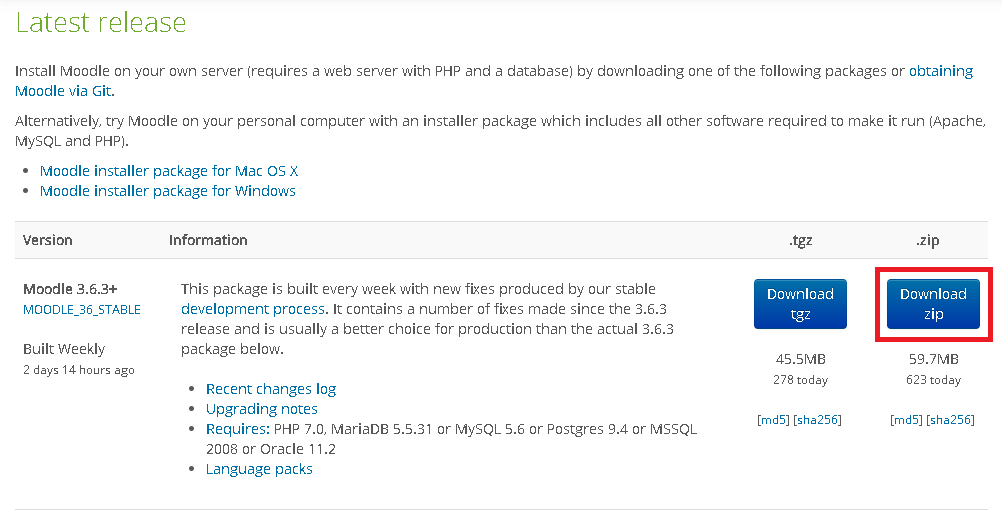
\includegraphics[width=0.8\linewidth]{img/packagemoodle}
		\end{center}
		\caption{Gói cài đặt Moodle 3.6.3+}
		\label{refhinh28}
	\end{figure}
\end{center}

\vskip 10cm
\subsubsection*{Tạo một cơ sở dữ liệu có tên moodle trên phpMyAdmin}

\begin{center}
	\begin{figure}[htp]
		\begin{center}
			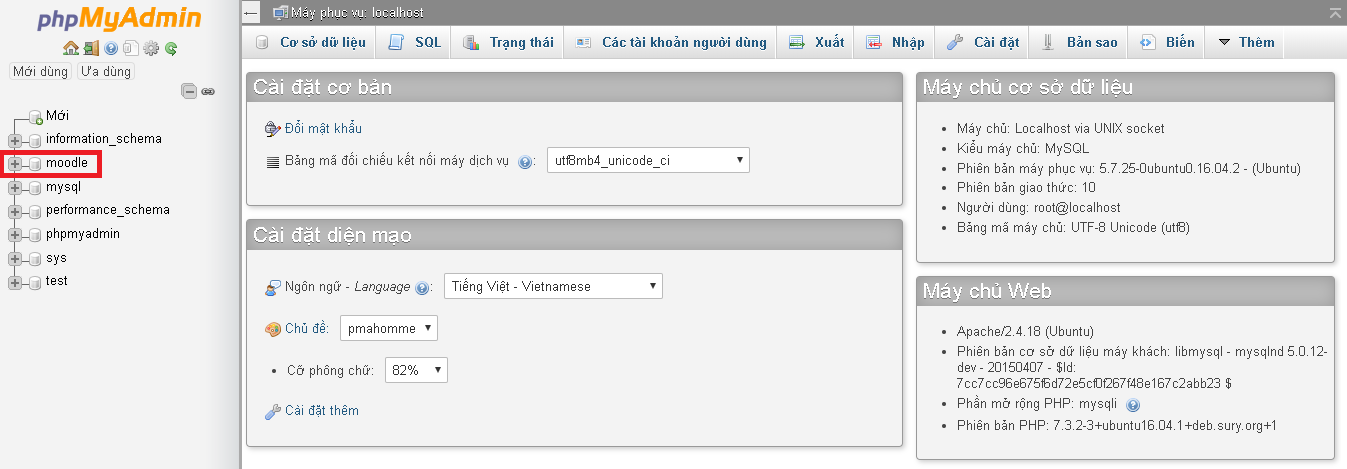
\includegraphics[width=1.3\linewidth]{img/dbmoodle}
		\end{center}
		\caption{Cơ sở dữ liệu moodle}
		\label{refhinh29}
	\end{figure}
\end{center}

\subsubsection*{Quá trình cài đặt Moodle}

\begin{center}
	\begin{figure}[htp]
		\begin{center}
			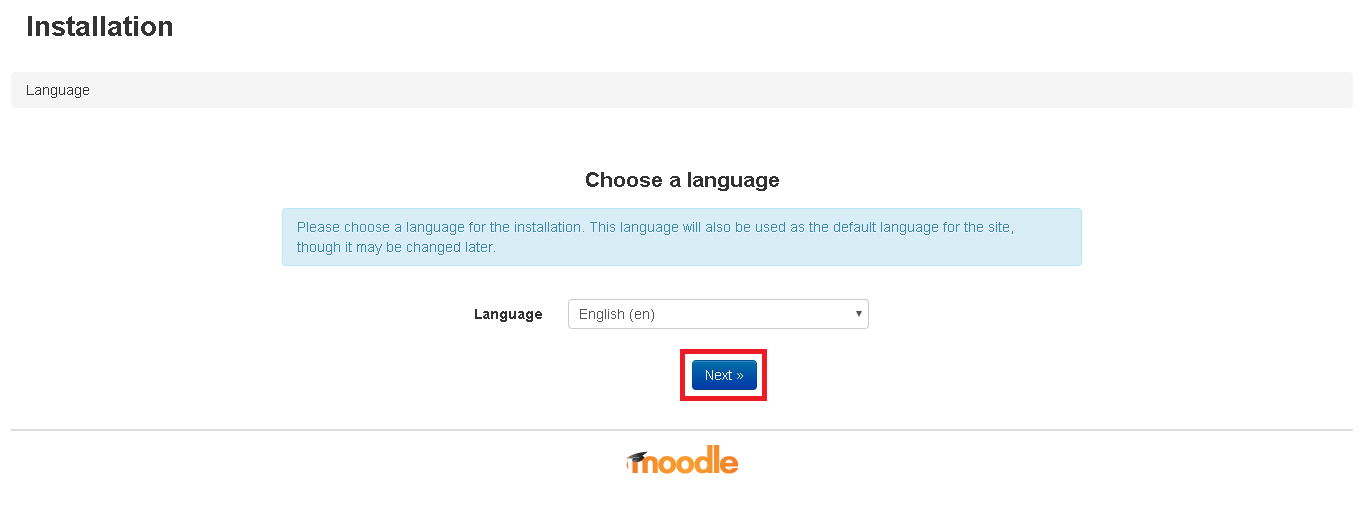
\includegraphics[width=1\linewidth]{img/choosenn}
		\end{center}
		\caption{Chọn ngôn ngữ cho Moodle}
		\label{refhinh30}
	\end{figure}
\end{center}

\begin{center}
	\begin{figure}[htp]
		\begin{center}
			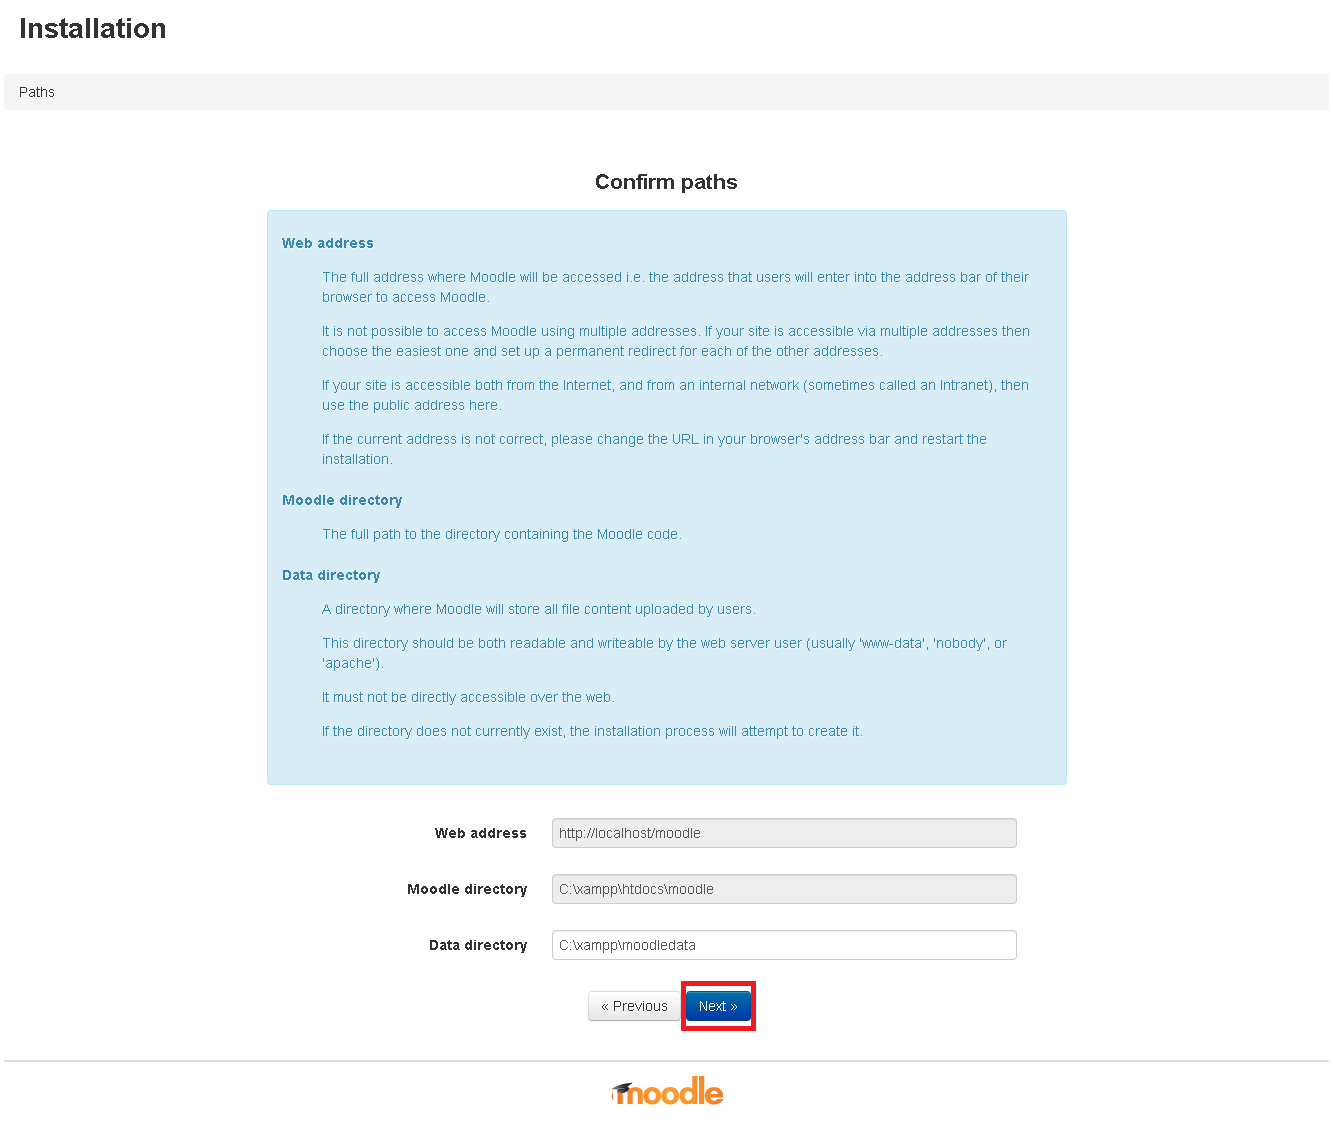
\includegraphics[width=0.8\linewidth]{img/direct}
		\end{center}
		\caption{Xác định lại các địa chỉ}
		\label{refhinh31}
	\end{figure}
\end{center}

\begin{center}
	\begin{figure}[htp]
		\begin{center}
			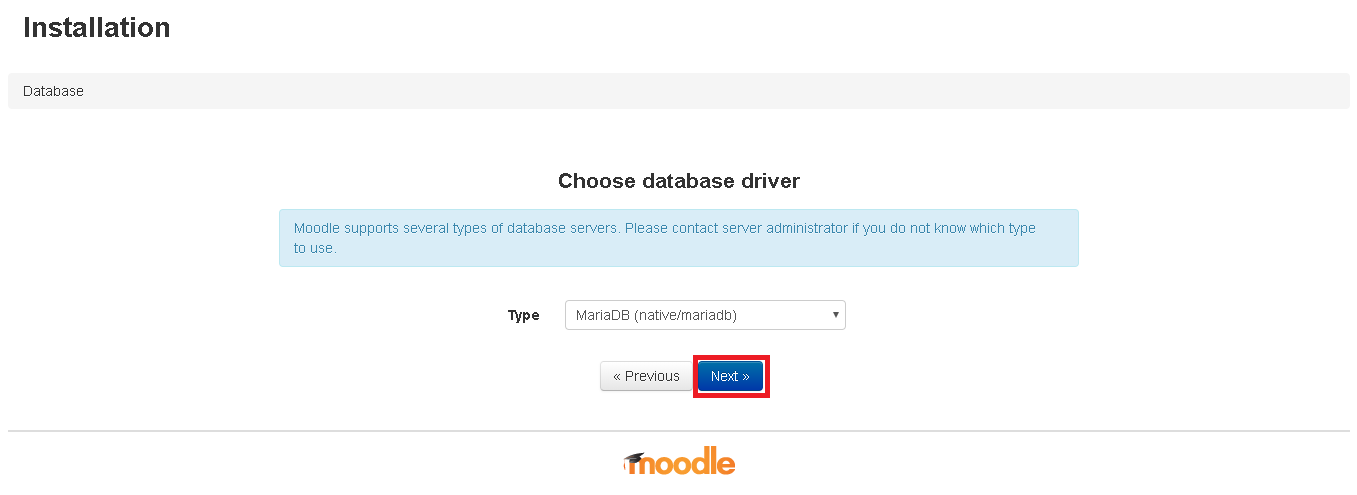
\includegraphics[width=1\linewidth]{img/2}
		\end{center}
		\caption{Chọn loại cơ sở dữ liệu}
		\label{refhinh32}
	\end{figure}
\end{center}

\begin{center}
	\begin{figure}[htp]
		\begin{center}
			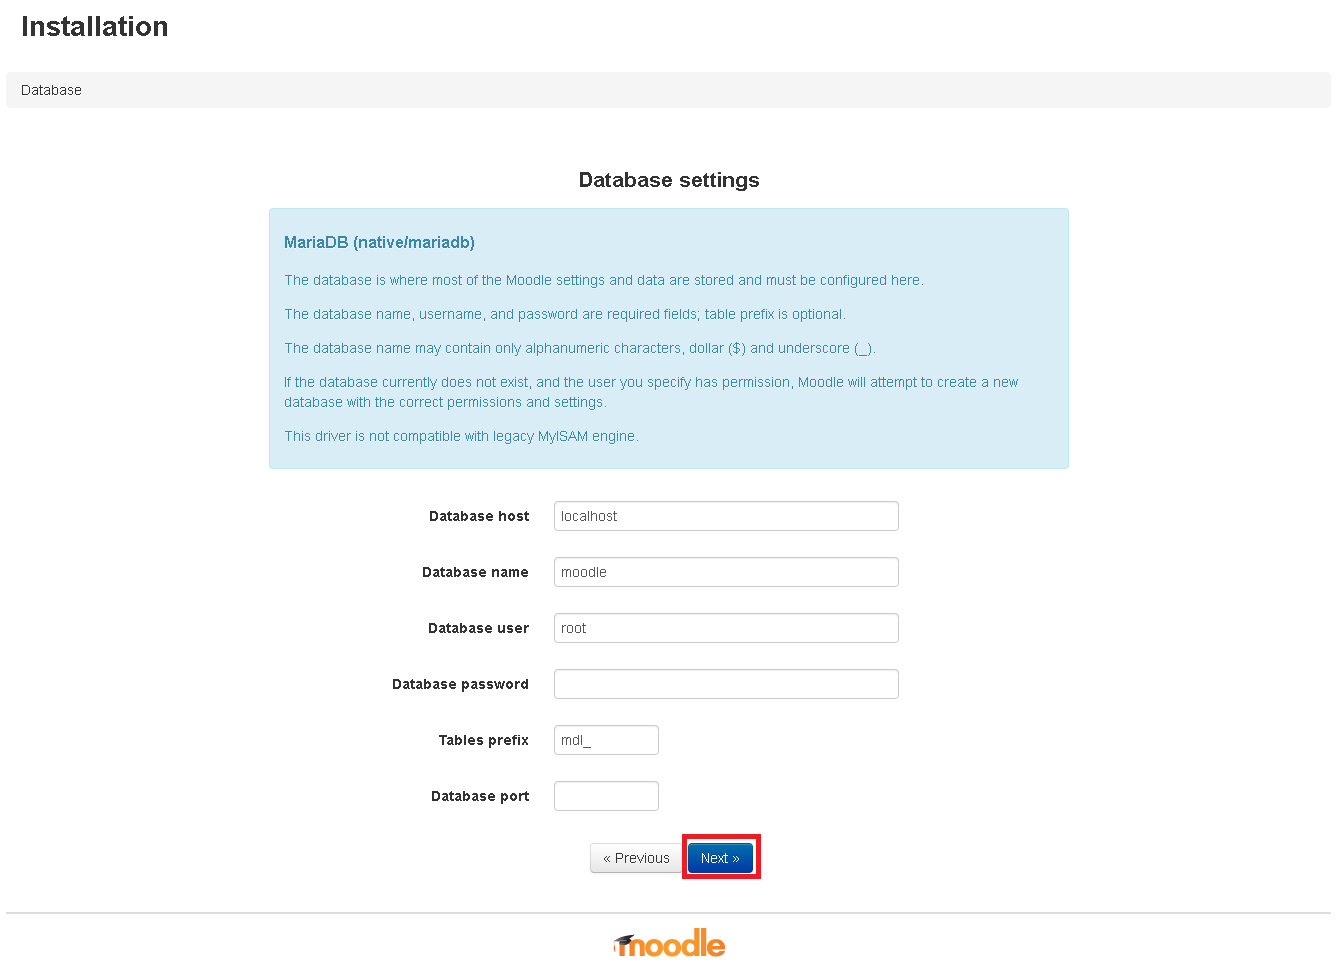
\includegraphics[width=1\linewidth]{img/3}
		\end{center}
		\caption{Cấu hình cơ sở dữ liệu}
		\label{refhinh33}
	\end{figure}
\end{center}

\begin{center}
	\begin{figure}[htp]
		\begin{center}
			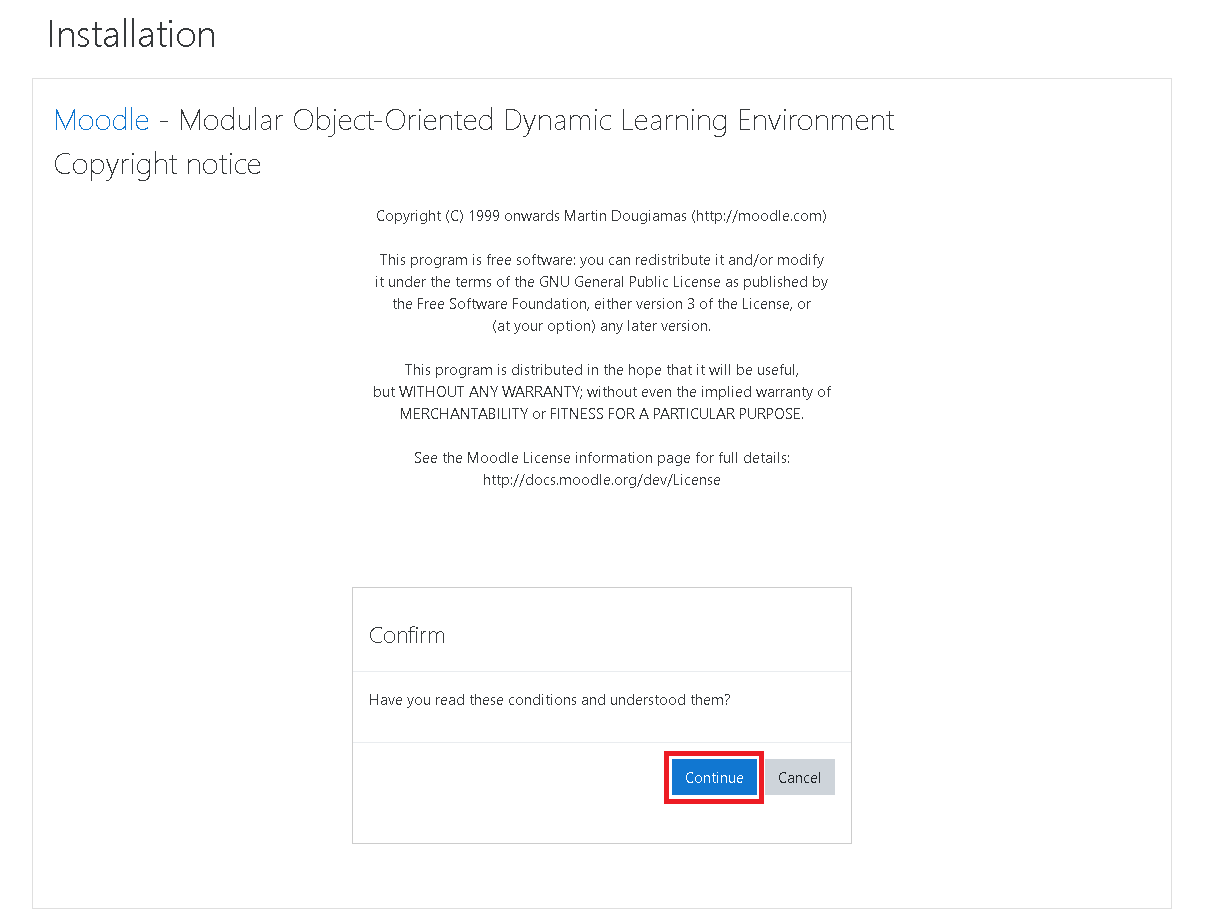
\includegraphics[width=0.8\linewidth]{img/4}
		\end{center}
		\caption{Điều kiện của Moodle}
		\label{refhinh34}
	\end{figure}
\end{center}

\begin{center}
	\begin{figure}[htp]
		\begin{center}
			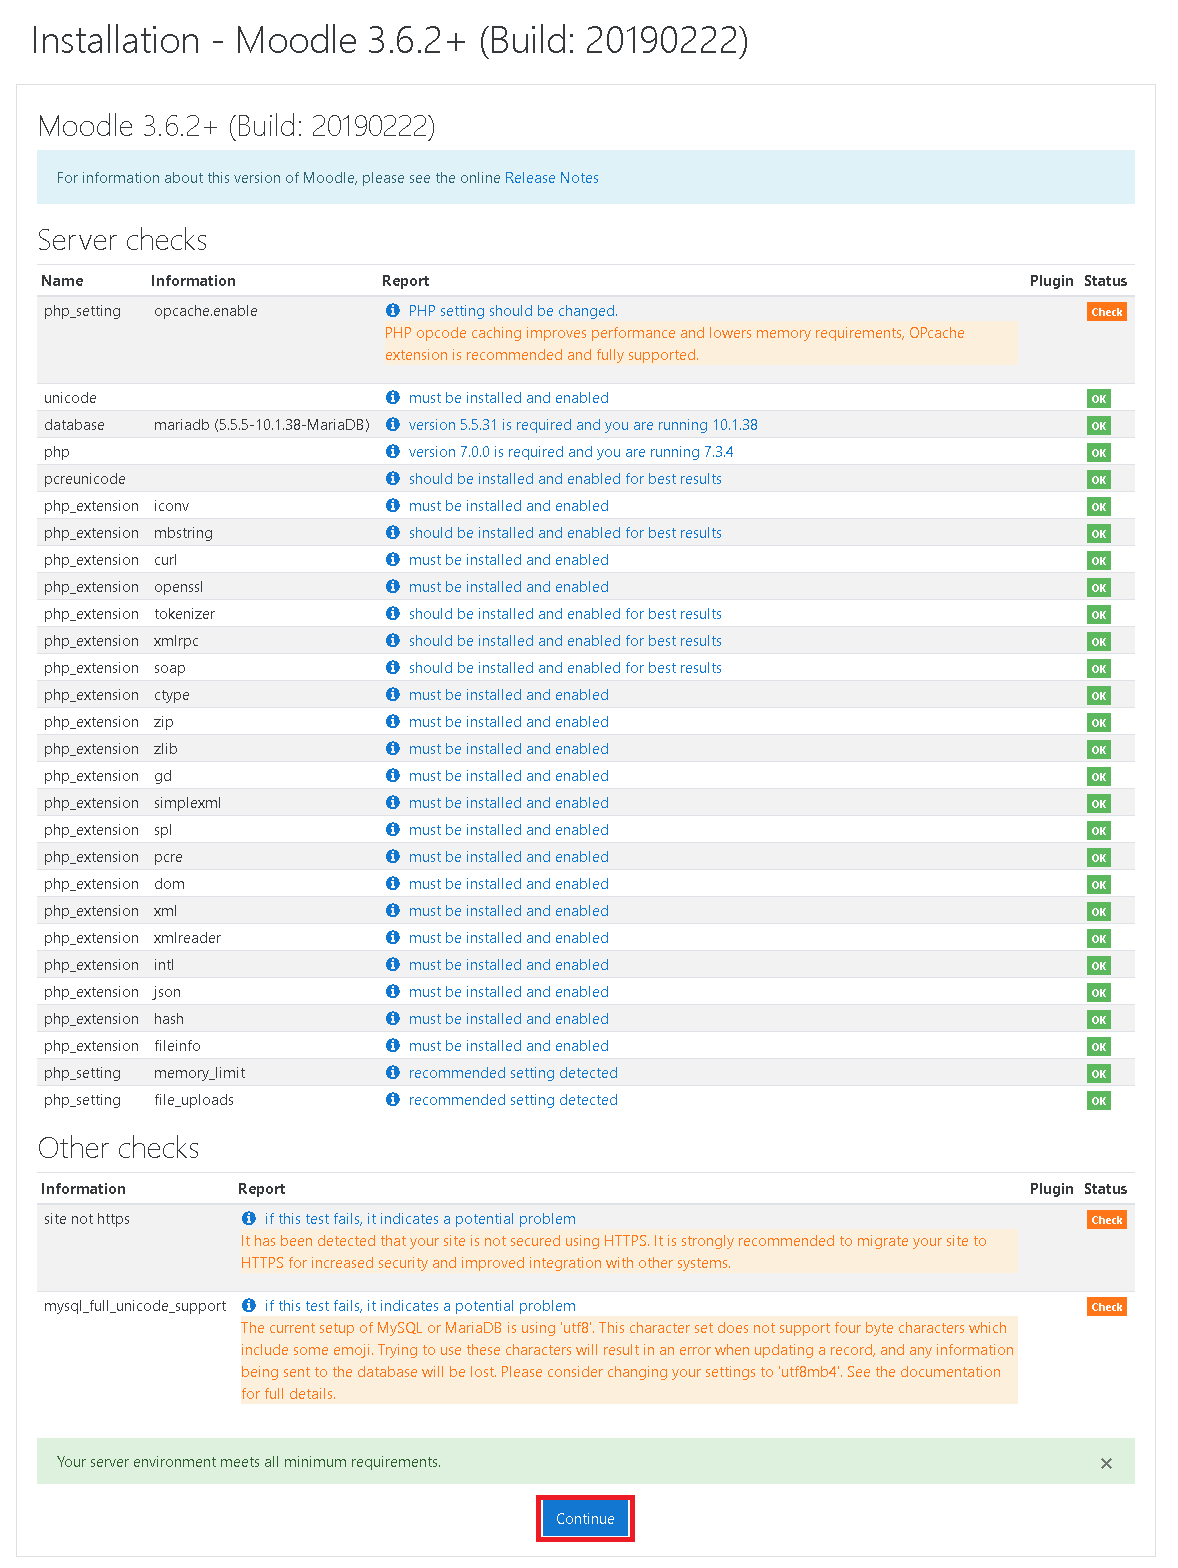
\includegraphics[width=0.65\linewidth]{img/5}
		\end{center}
		\caption{Kiểm tra server}
		\label{refhinh35}
	\end{figure}
\end{center}

\vskip 7cm
Chờ trong giây lát quá trình cài đặt Moodle sẽ hoàn thành.

\subsection*{Cài đặt Khối EHAT}
Tiếp theo nhóm sẽ giới thiệu quá trình cài đặt công cụ EHAT. Hãy kiểm tra lại lần nữa là Moodle của bạn đã được cài đặt và hoạt động bình thường nếu vẫn chưa cài Moodle thì hãy xem lại mục 4.3.1. Quá trình cài đặt sẽ được mô tả theo các bước sau:

\begin{itemize}
	\item Tại giao diện chính của trang chủ chọn mục Quản trị hệ thống(Đăng nhập Moodle với quyền Admin).
	
	\begin{center}
		\begin{figure}[htp]
			\begin{center}
				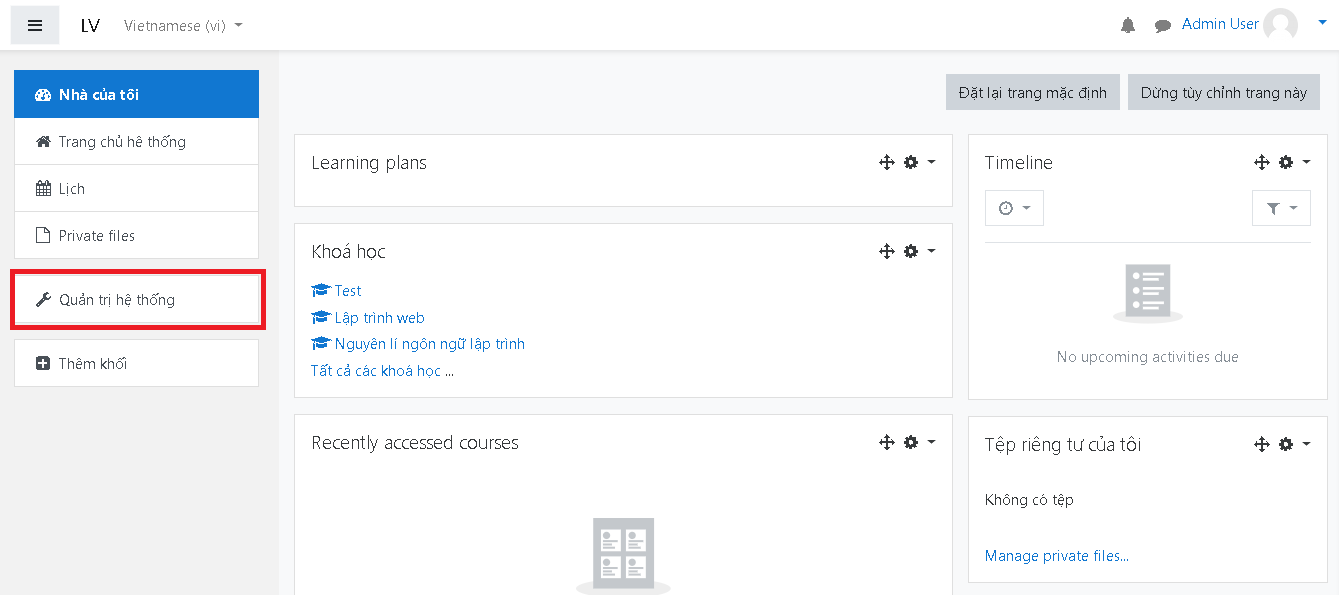
\includegraphics[width=1\linewidth]{img/6}
			\end{center}
			\caption{Chọn chức năng quản trị hệ thống}
			\label{refhinh36}
		\end{figure}
	\end{center}
	
	\item Tại trang Quản trị hệ thống người dùng chọn mục Module và chọn Install plugins
	
	\begin{center}
		\begin{figure}[htp]
			\begin{center}
				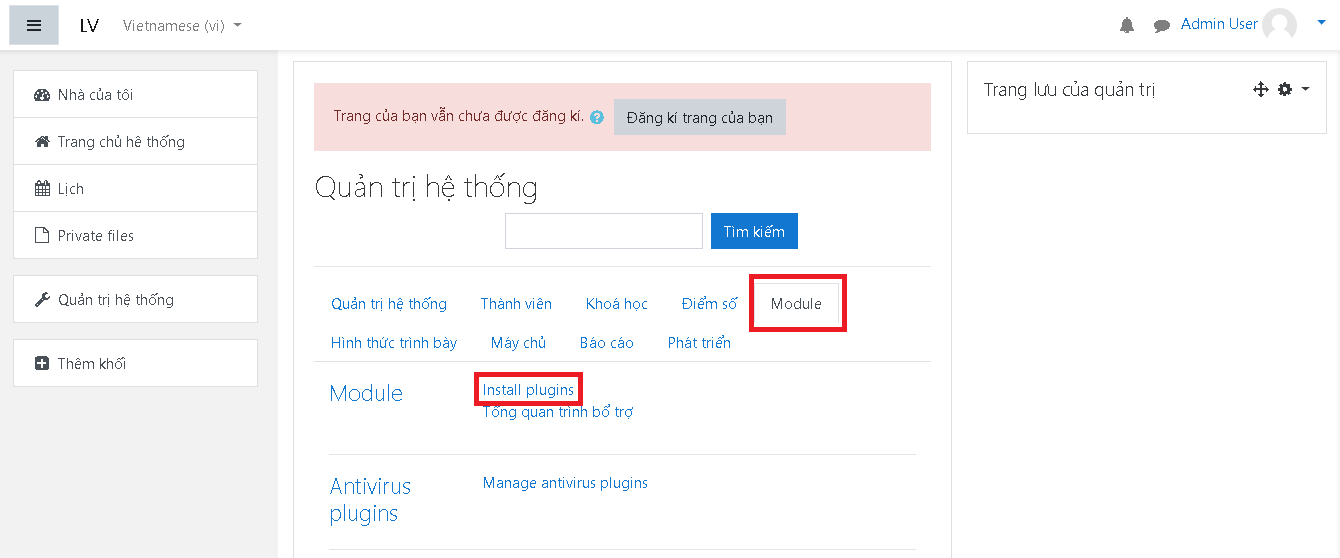
\includegraphics[width=1\linewidth]{img/7}
			\end{center}
			\caption{Chọn install plugins}
			\label{refhinh37}
		\end{figure}
	\end{center}
	
	\newpage
	\item Kéo thả tệp tin chứa công cụ EHAT(Định dạng file .zip).
	
	\begin{center}
		\begin{figure}[htp]
			\begin{center}
				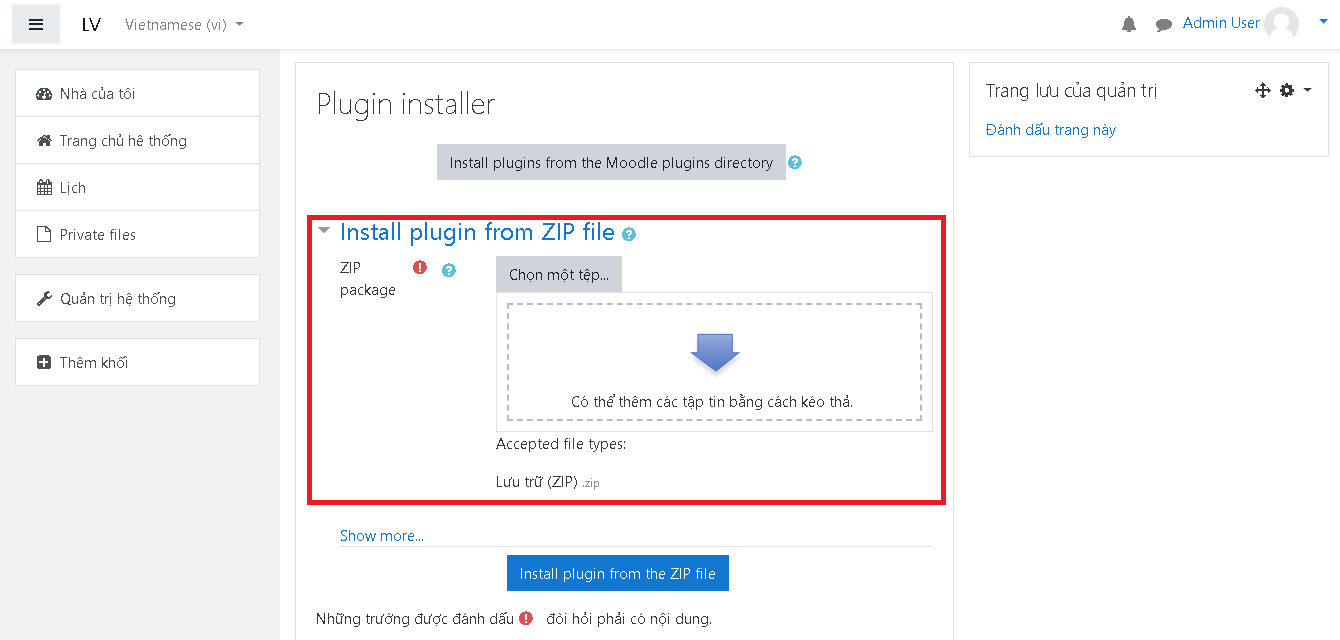
\includegraphics[width=1\linewidth]{img/8}
			\end{center}
			\caption{Chọn tệp tin chứa công cụ EHAT}
			\label{refhinh38}
		\end{figure}
	\end{center}
	
	\item Chọn Install plugin để tiếp tục.
	
	\begin{center}
		\begin{figure}[htp]
			\begin{center}
				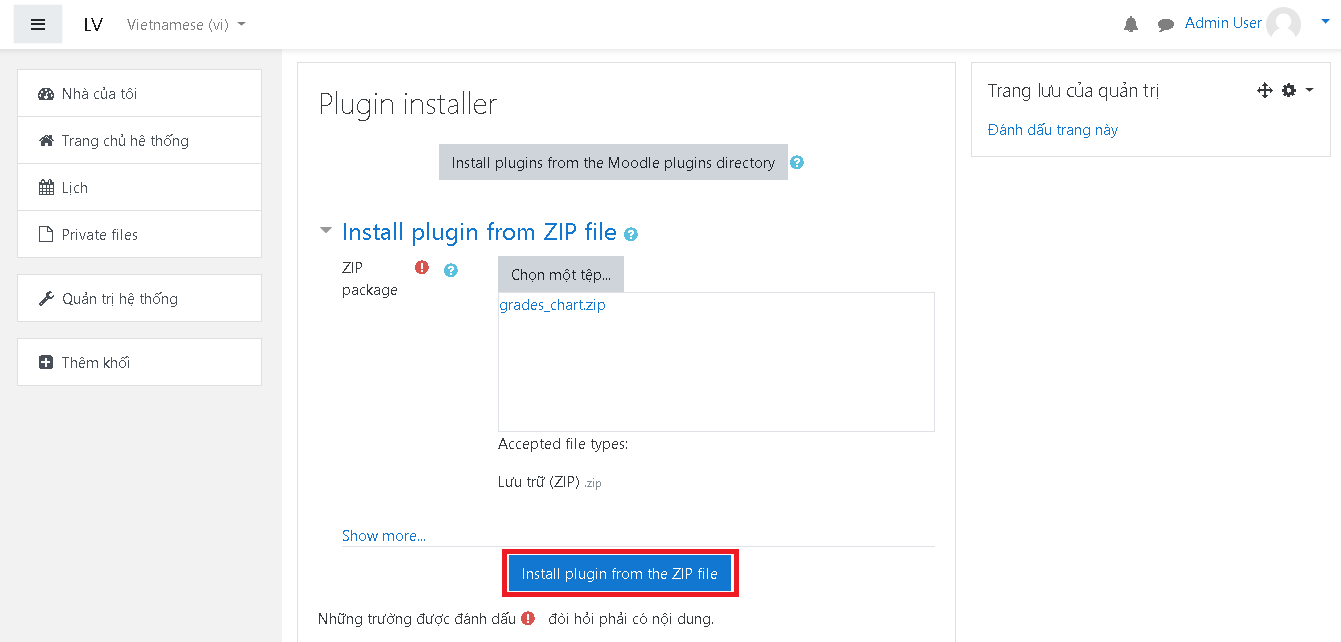
\includegraphics[width=1\linewidth]{img/9}
			\end{center}
			\caption{Chọn Install plugin để tiếp tục}
			\label{refhinh39}
		\end{figure}
	\end{center}
	
	\newpage
	\item Tiếp tục để cài đặt công cụ.
	
	\begin{center}
		\begin{figure}[htp]
			\begin{center}
				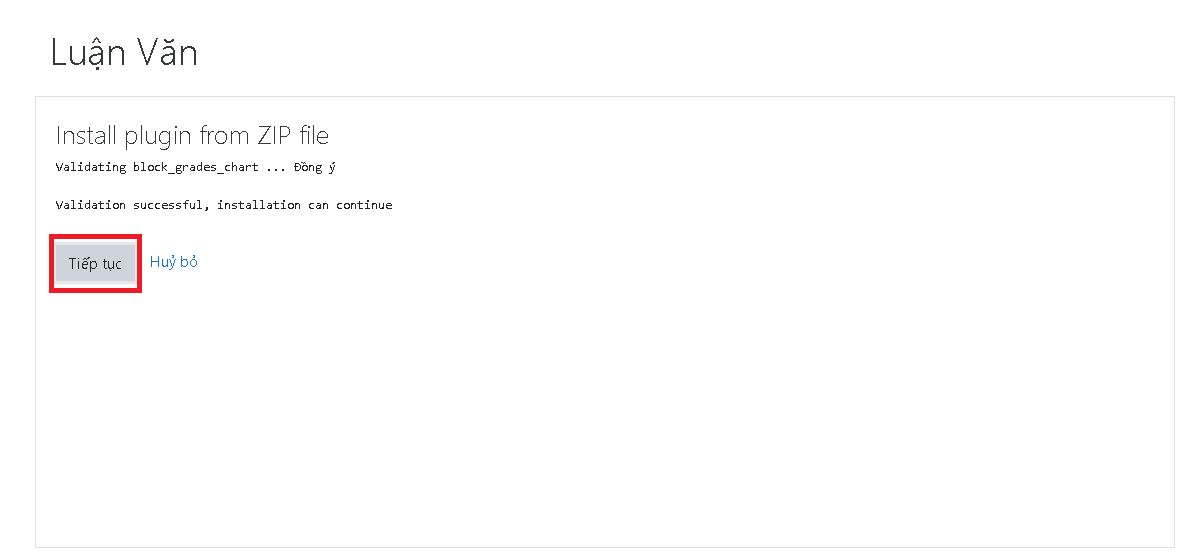
\includegraphics[width=1\linewidth]{img/10}
			\end{center}
			\caption{Chọn tiếp tục}
			\label{refhinh40}
		\end{figure}
	\end{center}
	
	\item Nâng cấp cơ sở dữ liệu Moodle để hoàn tất quá trình cài đặt
	
	\begin{center}
		\begin{figure}[htp]
			\begin{center}
				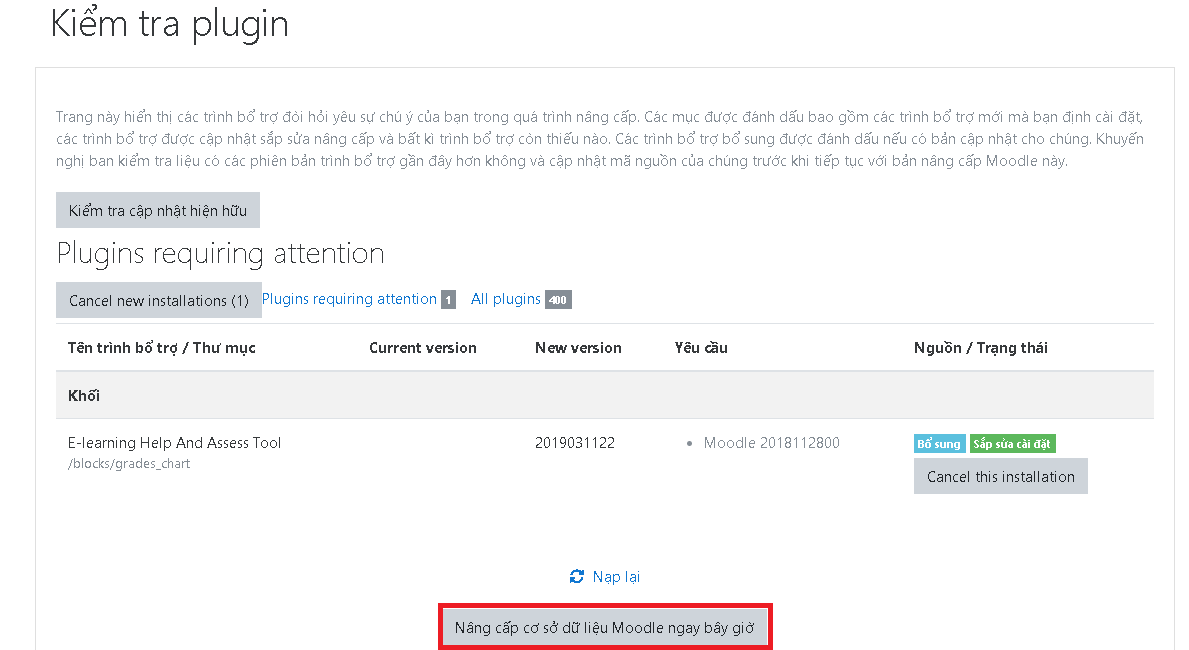
\includegraphics[width=1\linewidth]{img/11}
			\end{center}
			\caption{Giao diện nâng cấp cơ sở dữ liệu}
			\label{refhinh41}
		\end{figure}
	\end{center}
	
	\vskip 5cm
	\item Hoàn tất quá trình cài đặt EHAT
	
	\begin{center}
		\begin{figure}[htp]
			\begin{center}
				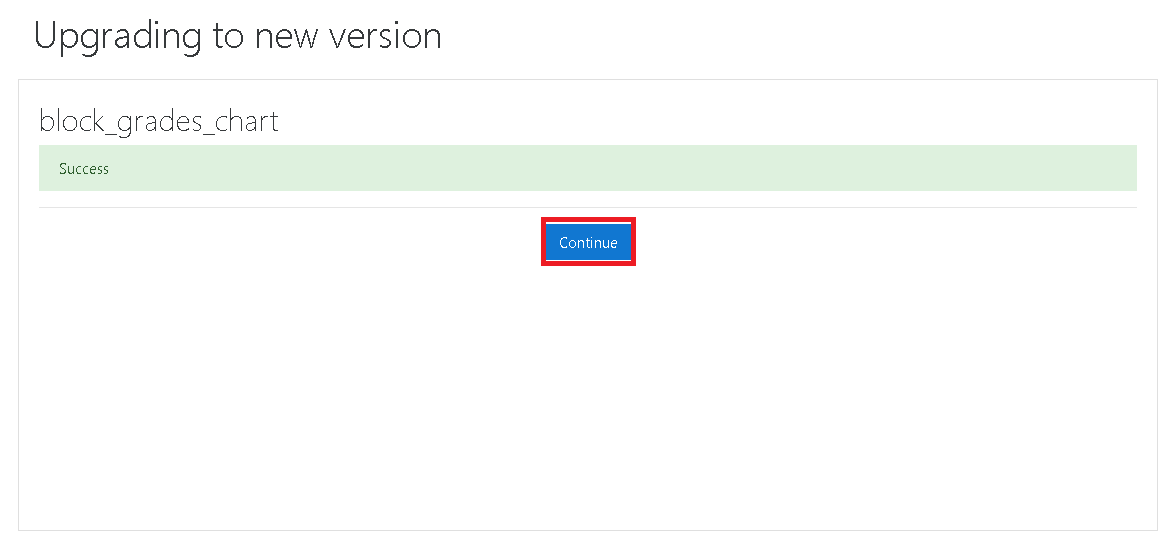
\includegraphics[width=1\linewidth]{img/12}
			\end{center}
			\caption{Quá trình cài đặt hoàn thành}
			\label{refhinh42}
		\end{figure}
	\end{center}
	
\end{itemize}


\subsection*{Các chức năng của EHAT đối với GV}

Đầu tiên để thấy được các chức năng của EHAT chúng ta cần thêm công cụ EHAT vào một khóa học mà ta muốn phân tích.

Ở giao diện trang chủ của Moodle ta chọn khóa học mà mình muốn thêm công cụ EHAT.

\begin{center}
	\begin{figure}[htp]
		\begin{center}
			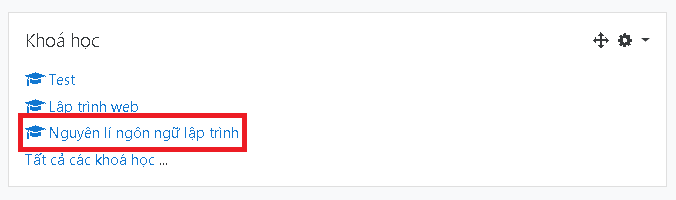
\includegraphics[width=1\linewidth]{img/35}
		\end{center}
		\caption{Chọn khóa học muốn phân tích}
		\label{refhinh43}
	\end{figure}
\end{center}

\newpage
Bật chế độ chỉnh sửa trong khóa học và chọn mục Thêm khối.

\begin{center}
	\begin{figure}[htp]
		\begin{center}
			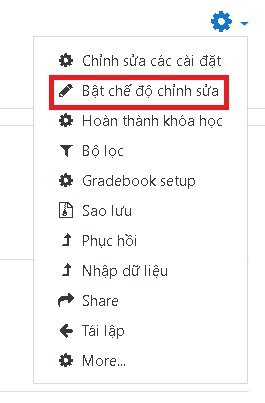
\includegraphics[width=0.4\linewidth]{img/36}
		\end{center}
		\caption{Bật chế độ chỉnh sửa}
		\label{refhinh44}
	\end{figure}
\end{center}

\begin{center}
	\begin{figure}[htp]
		\begin{center}
			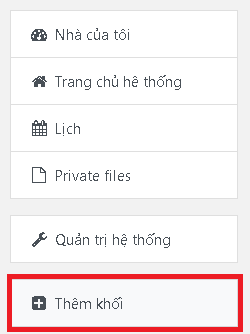
\includegraphics[width=0.35\linewidth]{img/38}
		\end{center}
		\caption{Chọn Thêm khối}
		\label{refhinh46}
	\end{figure}
\end{center}

\newpage
Chọn khối E-learning Help And Assess Tool

\begin{center}
	\begin{figure}[htp]
		\begin{center}
			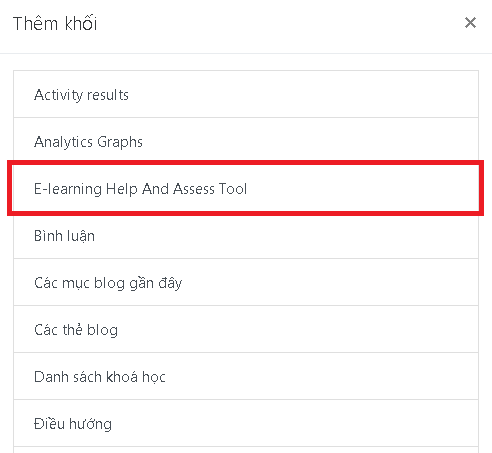
\includegraphics[width=0.6\linewidth]{img/37}
		\end{center}
		\caption{Chọn khối EHAT}
		\label{refhinh45}
	\end{figure}
\end{center}

Như vậy ta đã thêm công cụ EHAT vào khóa học.

\begin{center}
	\begin{figure}[htp]
		\begin{center}
			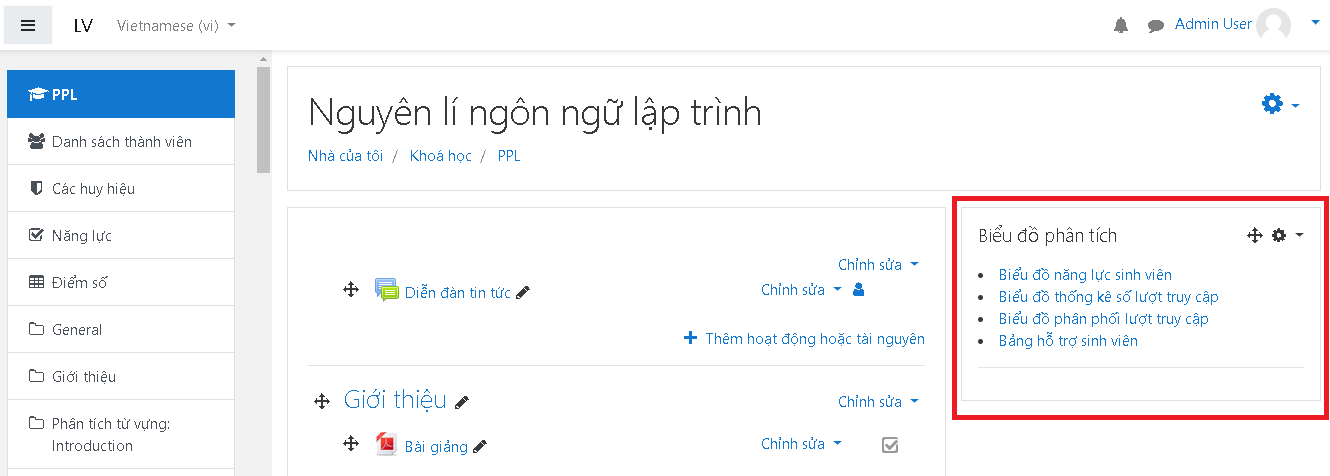
\includegraphics[width=1\linewidth]{img/39}
		\end{center}
		\caption{Thêm EHAT thành công}
		\label{refhinh47}
	\end{figure}
\end{center}

\newpage
\subsubsection*{Chức năng đánh giá năng lực SV}

Chúng ta cùng tìm hiểu giao diện của chức năng đầu tiên mà EHAT cung cấp cho GV.

\begin{center}
	\begin{figure}[htp]
		\begin{center}
			
\includegraphics[width=1\linewidth]{img/16}
		\end{center}
		\caption{Màn hình chính của chức năng thứ nhất}
		\label{refhinh48}
	\end{figure}
\end{center}

Nếu nhập số tiêu chí ít hơn 3 sẽ hiện thông báo lỗi.

\begin{center}
	\begin{figure}[htp]
		\begin{center}
			
\includegraphics[width=1\linewidth]{img/17}
		\end{center}
		\caption{Thông báo lỗi 1}
		\label{refhinh49}
	\end{figure}
\end{center}

\newpage
Nếu ta nhập đúng số tiêu chí thì giao diện sẽ chuyển sang màn hình mới.

\begin{center}
	\begin{figure}[htp]
		\begin{center}
			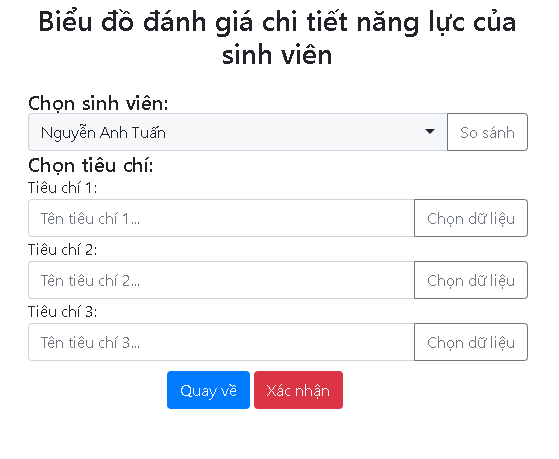
\includegraphics[width=0.6\linewidth]{img/18}
		\end{center}
		\caption{Màn hình thiết lập biểu đồ}
		\label{refhinh50}
	\end{figure}
\end{center}

Nếu ta không nhập tên tiêu chí hoặc thêm dữ liệu cho tiêu chí thì EHAT cũng sẽ báo lỗi.
\begin{center}
	\begin{figure}[htp]
		\begin{center}
			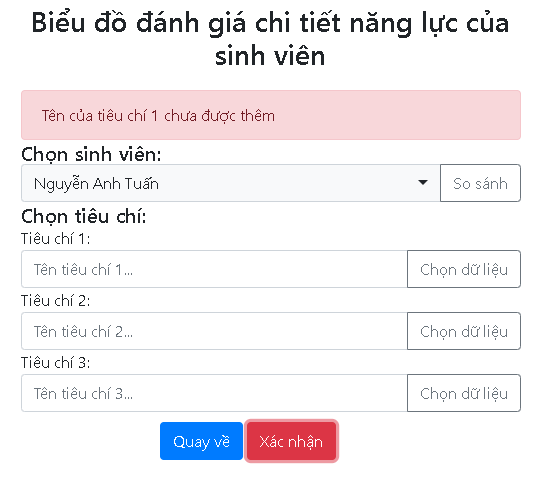
\includegraphics[width=0.6\linewidth]{img/19}
		\end{center}
		\caption{Thông báo lỗi 2}
		\label{refhinh51}
	\end{figure}
\end{center}

\begin{center}
	\begin{figure}[htp]
		\begin{center}
			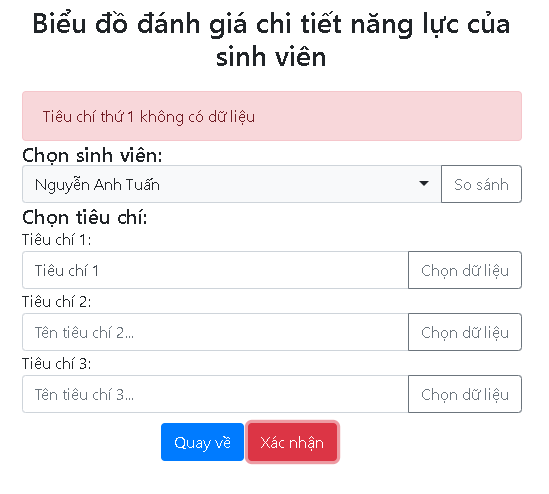
\includegraphics[width=0.6\linewidth]{img/20}
		\end{center}
		\caption{Thông báo lỗi 3}
		\label{refhinh52}
	\end{figure}
\end{center}

\vskip 5cm
Màn hình chọn dữ liệu cho tiêu chí.

\begin{center}
	\begin{figure}[htp]
		\begin{center}
			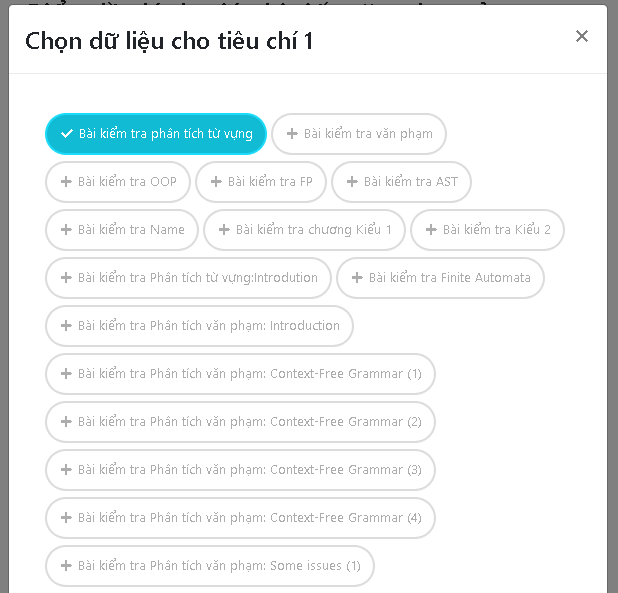
\includegraphics[width=0.5\linewidth]{img/21}
		\end{center}
		\caption{Giao diện chọn dữ liệu}
		\label{refhinh53}
	\end{figure}
\end{center}

\newpage
Sau khi đã hoàn tất mọi yêu cầu, chọn sinh viên cần tham khảo và nhấn nút xác nhận để xem biểu đồ năng lực của sinh viên đó.

\begin{center}
	\begin{figure}[htp]
		\begin{center}
			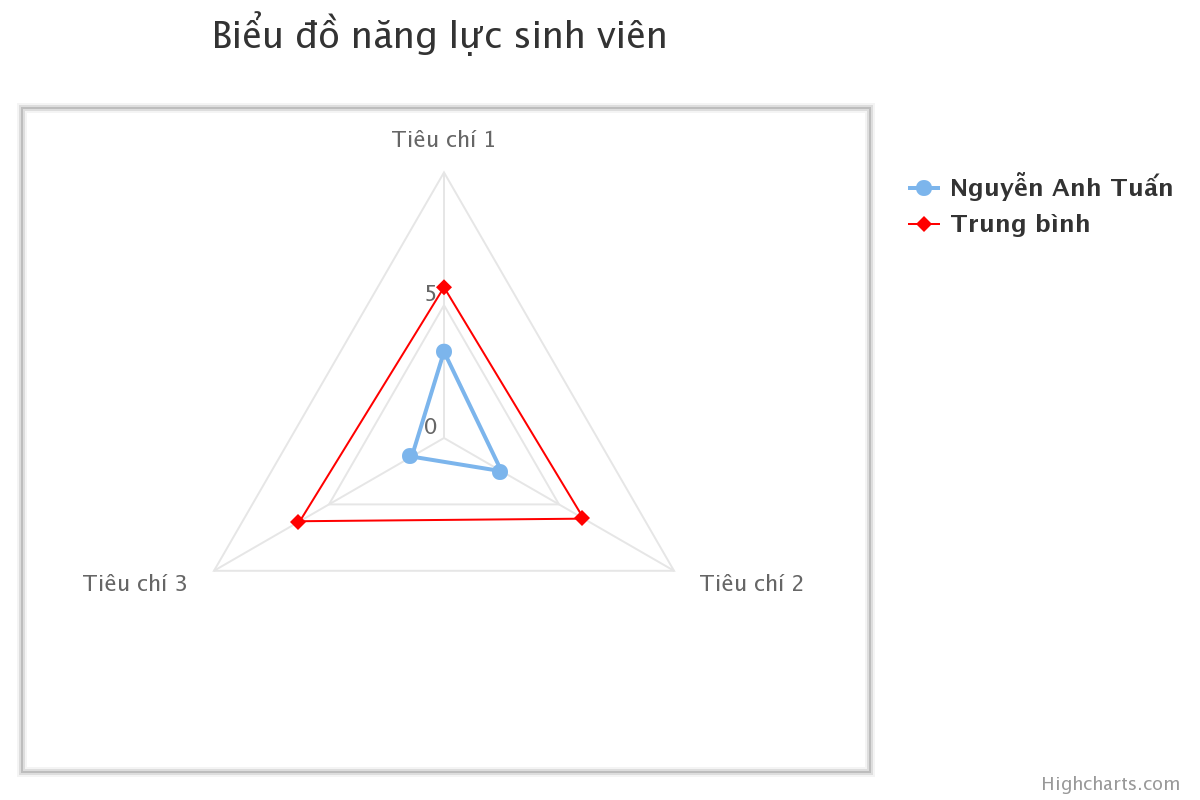
\includegraphics[width=1\linewidth]{img/22}
		\end{center}
		\caption{Biểu đồ năng lực sinh viên Nguyễn Anh Tuấn}
		\label{refhinh54}
	\end{figure}
\end{center}

\subsubsection*{Chức năng so sánh năng lực 2 SV}

Chọn nút So sánh nếu muốn so sánh 2 SV với nhau.

\begin{center}
	\begin{figure}[htp]
		\begin{center}
			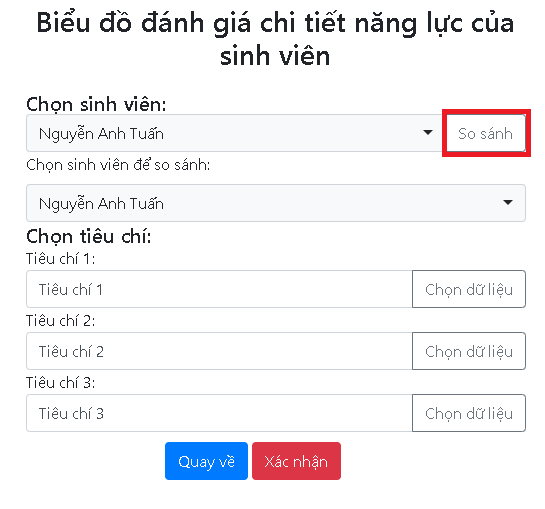
\includegraphics[width=0.4\linewidth]{img/23}
		\end{center}
		\caption{So sánh 2 SV}
		\label{refhinh55}
	\end{figure}
\end{center}
\vskip 3cm

Thông báo lỗi sẽ hiện ra nếu 2 SV so sánh là như nhau.

\begin{center}
	\begin{figure}[htp]
		\begin{center}
			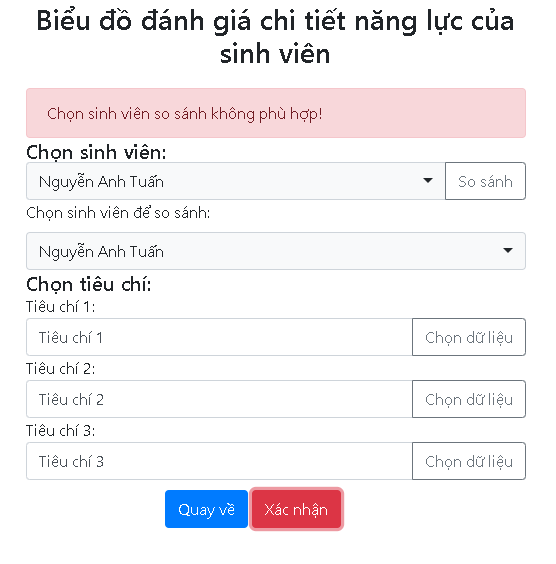
\includegraphics[width=0.5\linewidth]{img/24}
		\end{center}
		\caption{Thông báo lỗi 4}
		\label{refhinh56}
	\end{figure}
\end{center}

Sau khi chọn SV so sánh phù hợp nhấn nút xác nhận để thấy được biểu đồ so sánh 2 SV.
\begin{center}
	\begin{figure}[htp]
		\begin{center}
			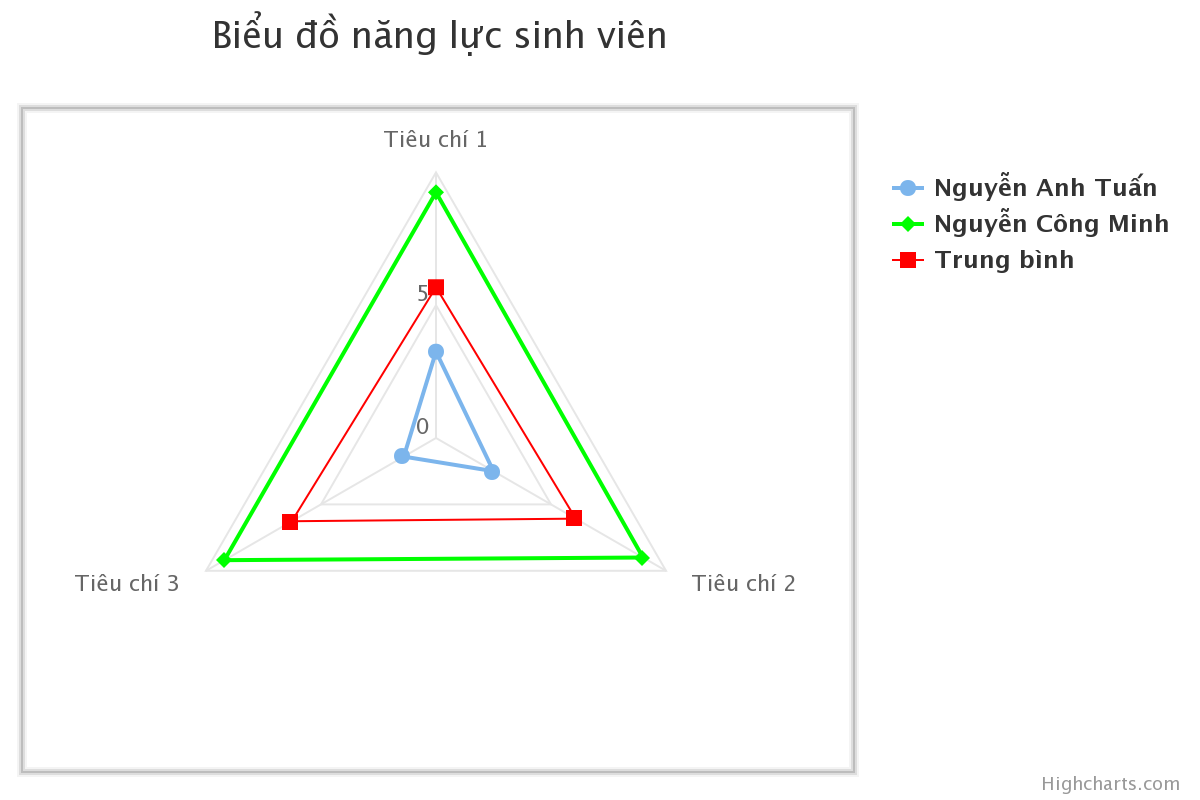
\includegraphics[width=0.8\linewidth]{img/25}
		\end{center}
		\caption{Biểu đồ so sánh năng lực 2 SV}
		\label{refhinh57}
	\end{figure}
\end{center}


\newpage
\subsubsection*{Biểu đồ thống kê số lượt truy cập của SV}

Giao diện chọn hạng mục để thống kê.

\begin{center}
	\begin{figure}[htp]
		\begin{center}
			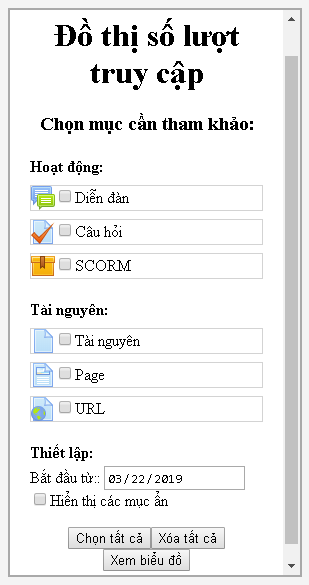
\includegraphics[width=0.6\linewidth]{img/26}
		\end{center}
		\caption{Chọn mục cần thống kê}
		\label{refhinh58}
	\end{figure}
\end{center}

\begin{center}
	\begin{figure}[htp]
		\begin{center}
			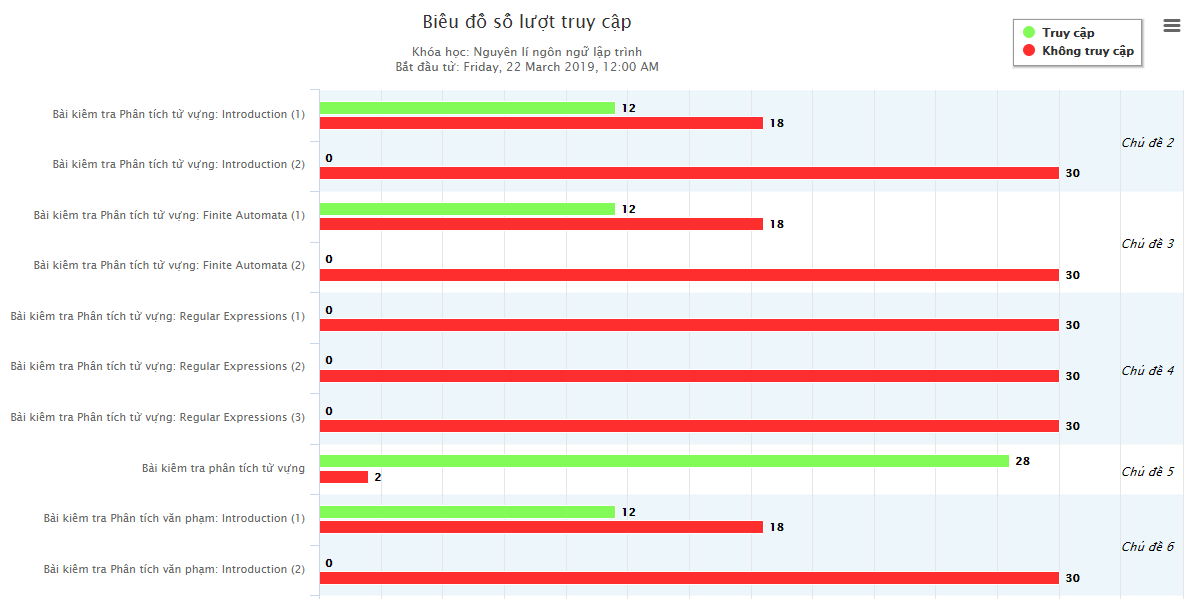
\includegraphics[width=1\linewidth]{img/27}
		\end{center}
		\caption{Biểu đồ thống kê số lượt truy cập của SV}
		\label{refhinh59}
	\end{figure}
\end{center}

\vskip 5cm
Xem chi tiết những sinh viên nào truy cập.

\begin{center}
	\begin{figure}[htp]
		\begin{center}
			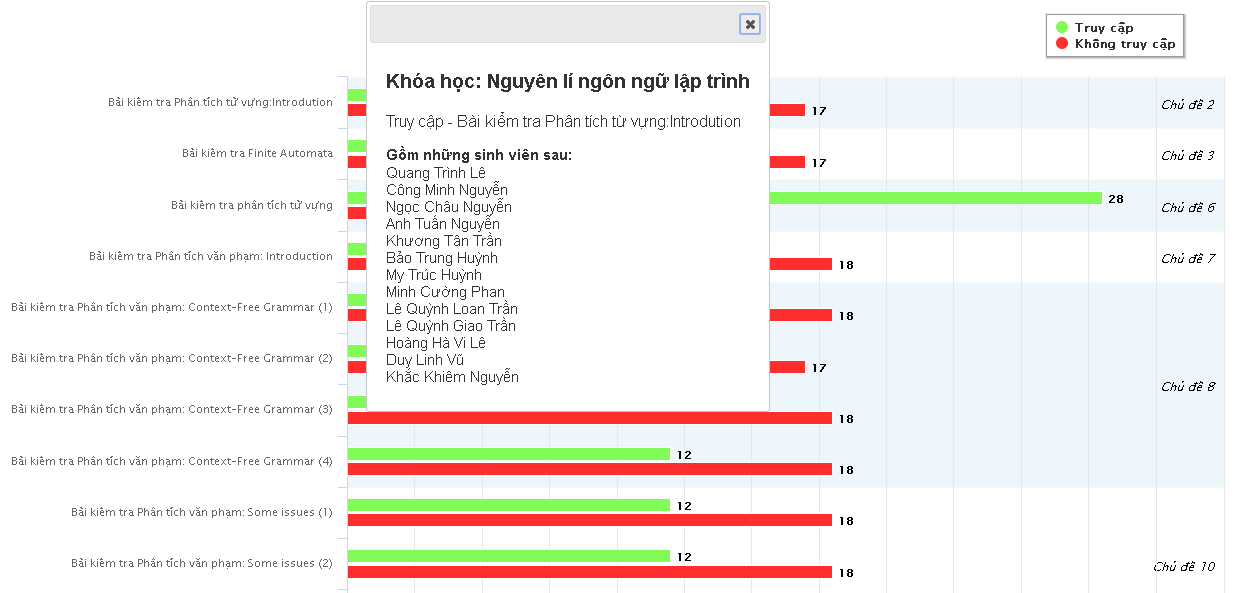
\includegraphics[width=1\linewidth]{img/28}
		\end{center}
		\caption{Chi tiết số sinh viên}
		\label{refhinh60}
	\end{figure}
\end{center}

\newpage
\subsubsection*{Biểu đồ phân phối lượt truy cập của SV}

Giao diện biểu đồ phân phối lượt truy cập của SV.

\begin{center}
	\begin{figure}[htp]
		\begin{center}
			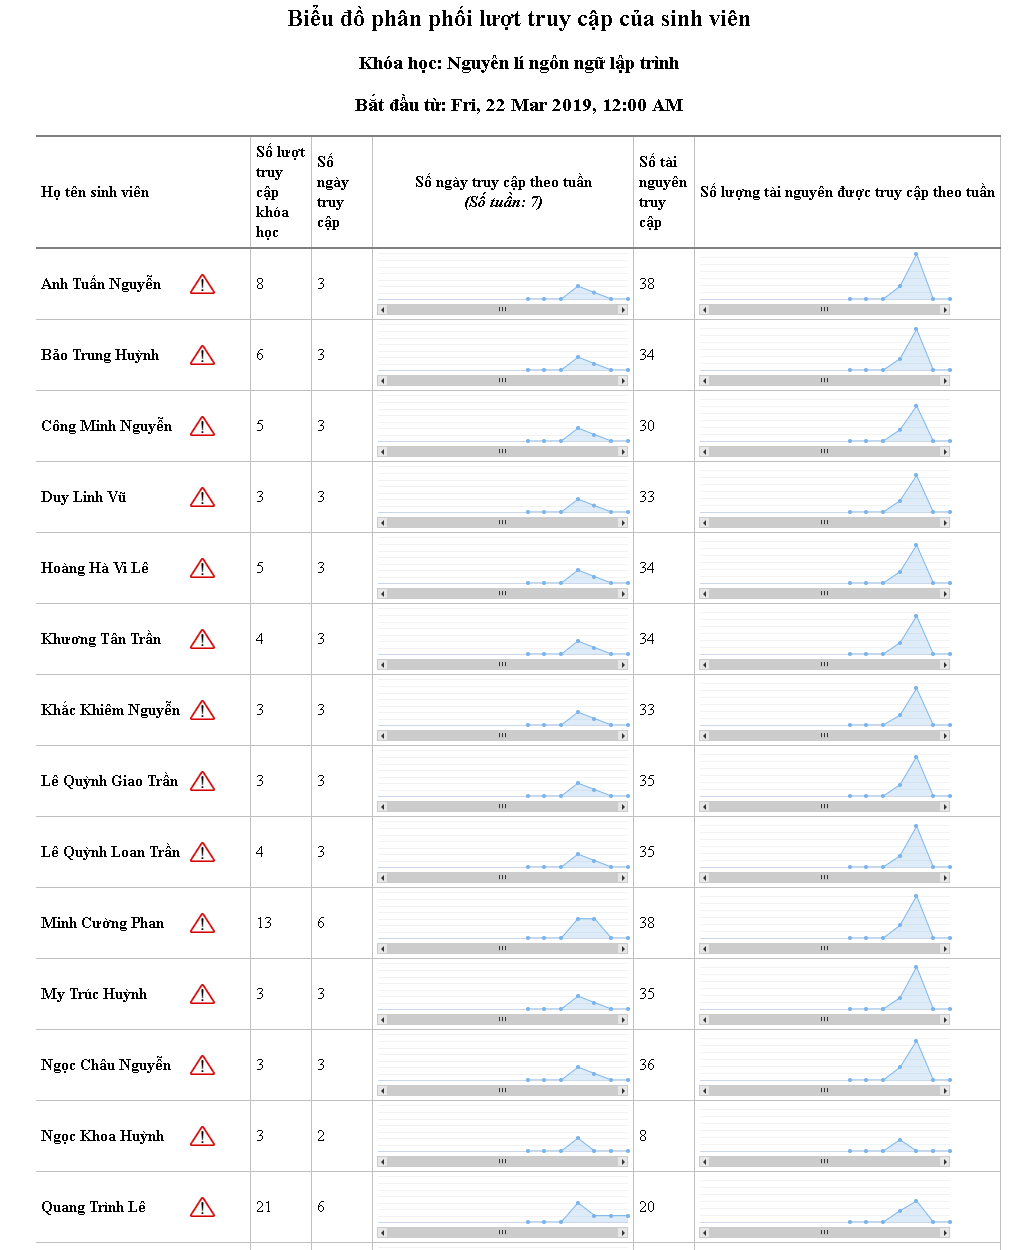
\includegraphics[width=1\linewidth]{img/29}
		\end{center}
		\caption{Giao diện biểu đồ phân phối lượt truy cập của SV}
		\label{refhinh61}
	\end{figure}
\end{center}

\newpage
Để xem chi tiết lượt truy cập của sinh viên nào ta cần nhấp chuột vào tên của sinh viên ấy.

\begin{center}
	\begin{figure}[htp]
		\begin{center}
			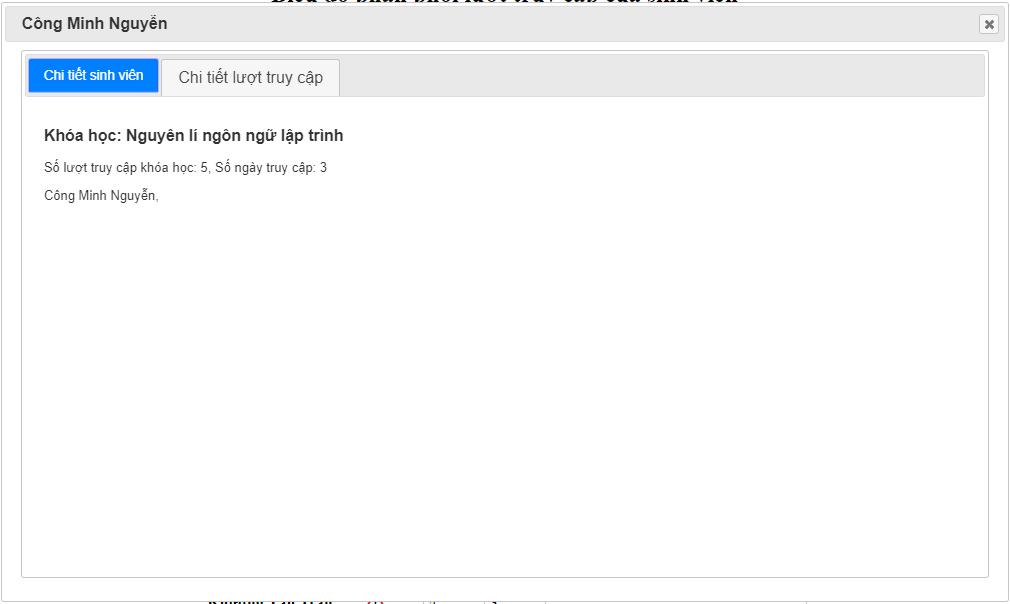
\includegraphics[width=0.9\linewidth]{img/40}
		\end{center}
		\caption{Giao diện chính xem chi tiết lượt truy cập của sinh viên}
		\label{refhinh67}
	\end{figure}
\end{center}

\begin{center}
	\begin{figure}[htp]
		\begin{center}
			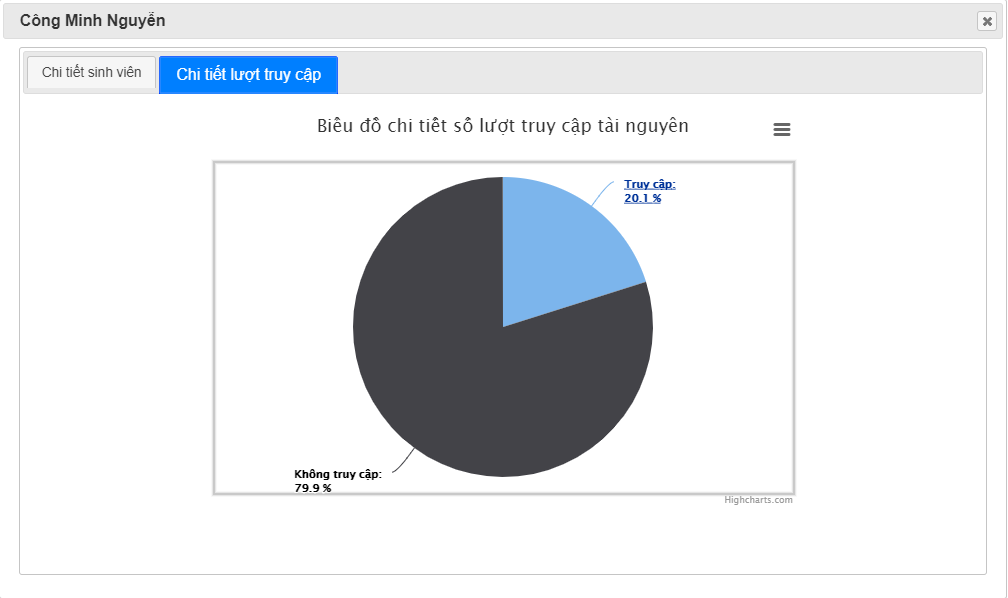
\includegraphics[width=0.9\linewidth]{img/41}
		\end{center}
		\caption{Biểu đồ phần trăm lượt truy cập của sinh viên}
		\label{refhinh68}
	\end{figure}
\end{center}

\begin{center}
	\begin{figure}[htp]
		\begin{center}
			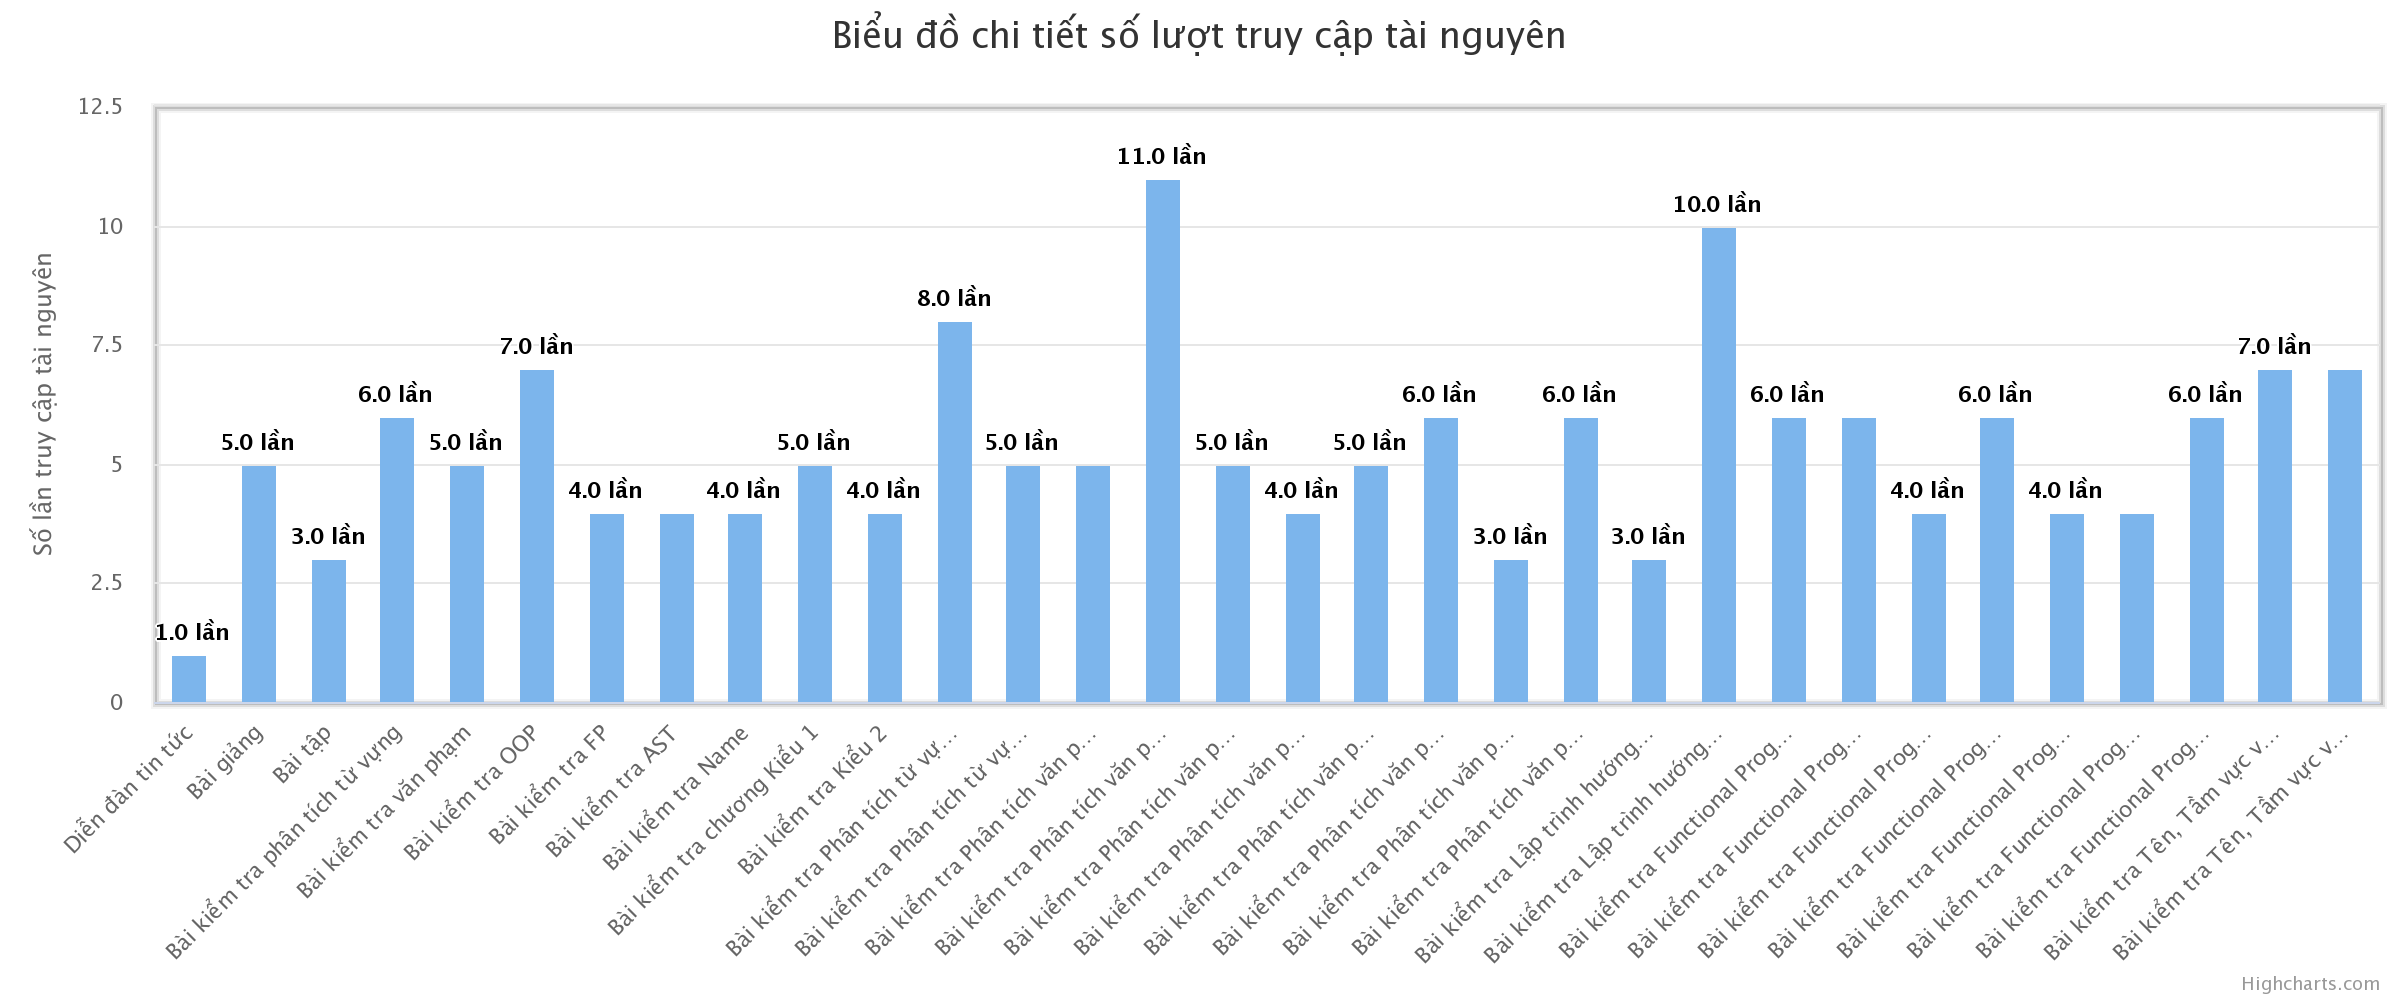
\includegraphics[width=1\linewidth]{img/42}
		\end{center}
		\caption{Biểu đồ chi tiết số lần truy cập của sinh viên}
		\label{refhinh69}
	\end{figure}
\end{center}

\newpage
\subsubsection*{Bảng thêm tài liệu tham khảo nhằm hỗ trợ sinh viên}

Giao diện bảng thêm tài liệu.

\begin{center}
	\begin{figure}[htp]
		\begin{center}
			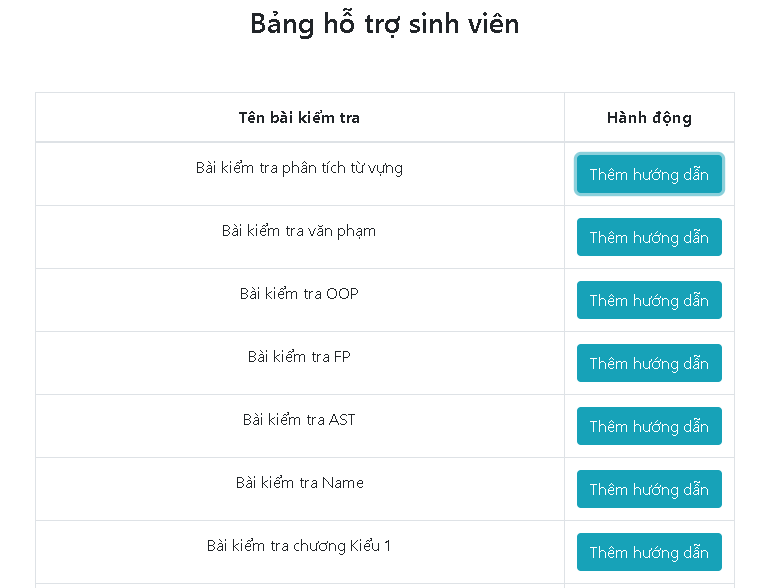
\includegraphics[width=0.6\linewidth]{img/30}
		\end{center}
		\caption{Giao diện bảng thêm tài liệu 1}
		\label{refhinh62}
	\end{figure}
\end{center}

\begin{center}
	\begin{figure}[htp]
		\begin{center}
			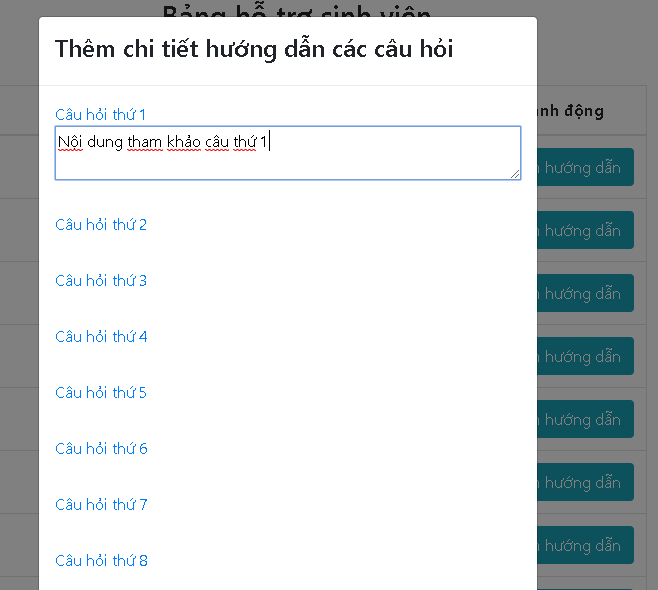
\includegraphics[width=0.6\linewidth]{img/31}
		\end{center}
		\caption{Giao diện bảng thêm tài liệu 2}
		\label{refhinh63}
	\end{figure}
\end{center}

\newpage
\subsection*{Các chức năng của EHAT đối với HS, SV}

Giao diện công cụ EHAT trên màn hình của HS, SV.

\begin{center}
	\begin{figure}[htp]
		\begin{center}
			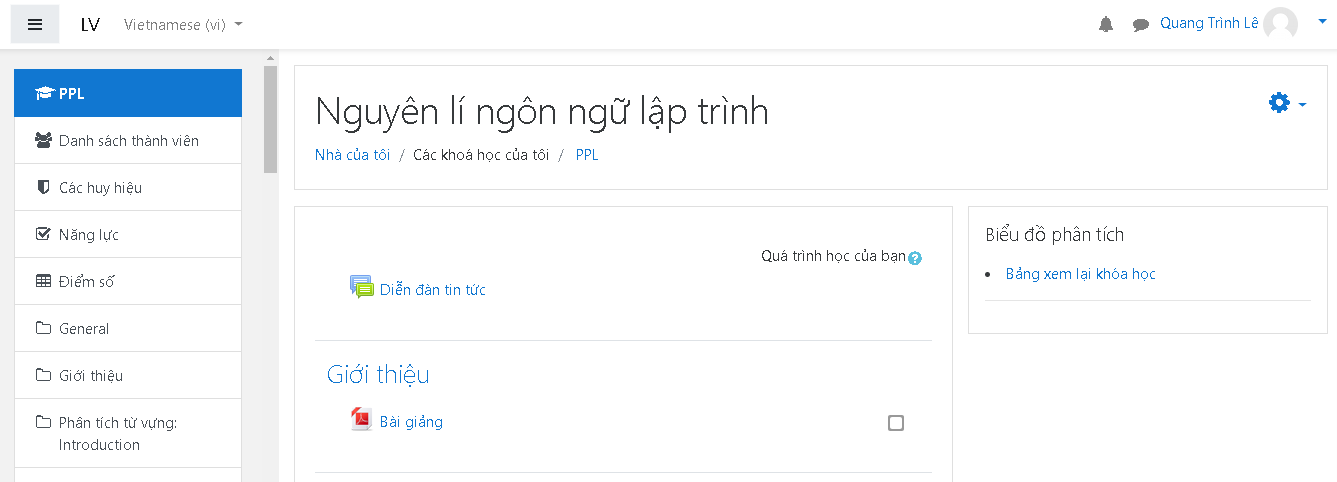
\includegraphics[width=1\linewidth]{img/32}
		\end{center}
		\caption{Giao diện công cụ EHAT trên màn hình của HS, SV}
		\label{refhinh64}
	\end{figure}
\end{center}

\newpage
\subsubsection*{Bảng xem lại khóa học của sinh viên}

\begin{center}
	\begin{figure}[htp]
		\begin{center}
			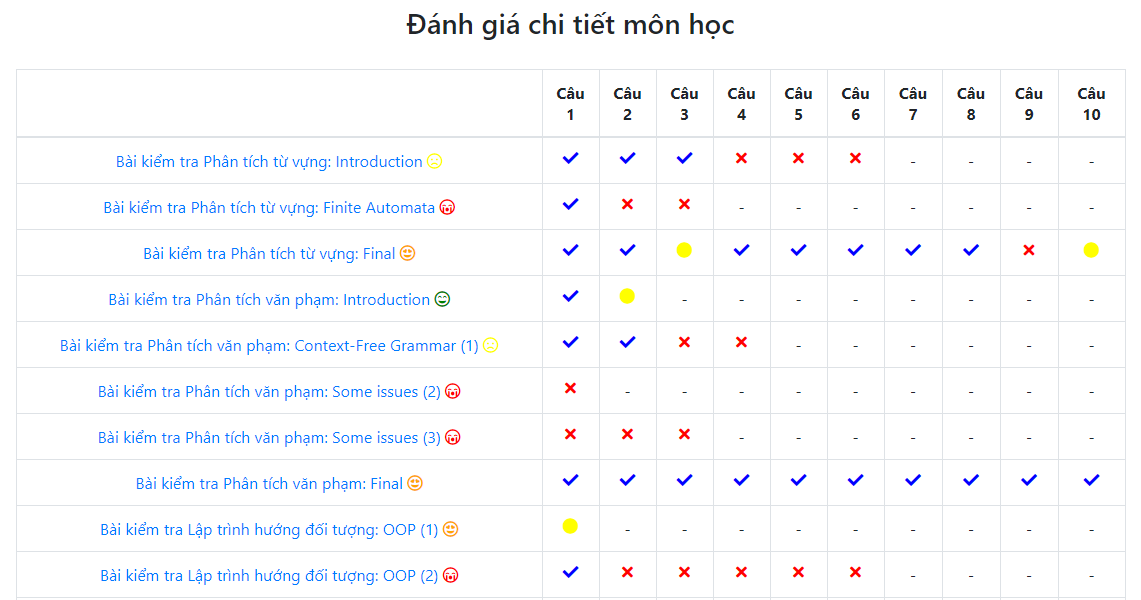
\includegraphics[width=1\linewidth]{img/33}
		\end{center}
		\caption{Bảng xem lại khóa học của sinh viên}
		\label{refhinh65}
	\end{figure}
\end{center}

Nội dung chi tiết của từng câu hỏi.

\begin{center}
	\begin{figure}[htp]
		\begin{center}
			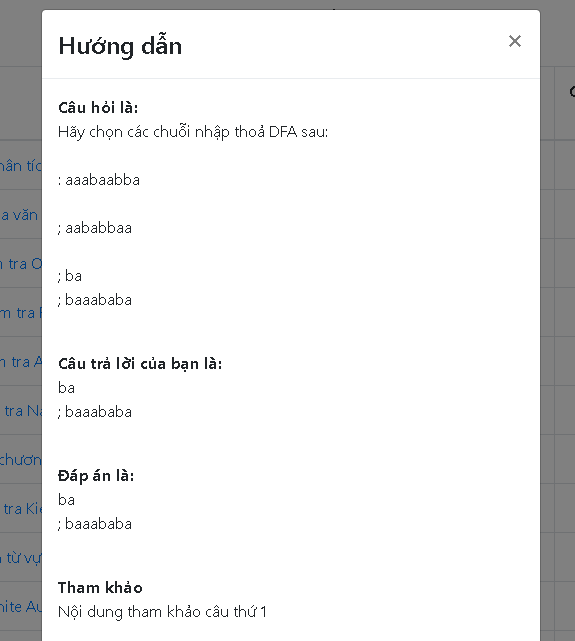
\includegraphics[width=0.5\linewidth]{img/34}
		\end{center}
		\caption{Nội dung chi tiết của từng câu hỏi}
		\label{refhinh66}
	\end{figure}
\end{center}